% Regenerate the figure before compiling:
%   py ../scripts/make_figures.py
% Compile from this directory:
%   tectonic -X compile main.tex
\documentclass[11pt]{article}

\usepackage[margin=1.1in]{geometry}
\usepackage{amsmath,amssymb}
\usepackage{booktabs}
\usepackage{graphicx}
\usepackage[font=small]{caption}
\usepackage{microtype}
\usepackage[round,authoryear]{natbib}
\usepackage{hyperref}

\hypersetup{
  colorlinks=true,
  allcolors=black,
  pdfauthor={Roman Mirosenski},
  pdftitle={How much of a backtest is the search},
  pdfsubject={Selection bias and structure dependence in backtested strategies},
  pdfkeywords={backtest overfitting, deflated Sharpe ratio, selection bias, block bootstrap}
}

\title{\textbf{How much of a backtest is the search?}\\[4pt]
\large Selection bias and structure dependence in backtested strategies}
\author{Roman Mirosenski\\[2pt]\small\texttt{github.com/RomanMski/overfitlab}}
\date{}

\begin{document}
\maketitle

\begin{abstract}
A backtest reports the best of everything you tried, and that number is biased upward by however hard you searched. Two published corrections exist for this and both are implemented here. Neither asks a second question that matters as much, which is whether the market held anything the strategy was reading at all.

That question has an obvious experiment behind it. Destroy the ordering of the return series, rerun the strategy, and see what survives. The obvious implementation is a block bootstrap, and it is wrong. Resampling with replacement drops some observations and duplicates others, so the generated path has a different realised distribution from the source and the experiment varies two things at once. On a 1500 point series, one bootstrap path was missing 549 of the distinct source values and 79 of 200 paths had lost the largest loss entirely.

A block permutation removes the confound. Every observation appears exactly once, so the empirical distribution is fixed by construction and only the arrangement varies. Sweeping the block length then separates a result that needs the ordering from one that would have happened in any ordering. On a simulated market with momentum, a trend follower earning 1.00 annualised falls to 0.00 once the ordering is destroyed and recovers as blocks lengthen, while buy and hold returns the source value at every block length to within one floating point unit, because its result depends only on the multiset of returns and a permutation cannot change that. Under a bootstrap the same quantity scatters with a standard deviation roughly as large as itself.

Run on daily prices for five liquid exchange traded funds since 2000, the size of that collapse and its statistical significance turn out to disagree in both directions. A 60 day trend follower loses half its Sharpe ratio to shuffling and still fails to beat a third of the shuffled markets, while volatility targeting, which expresses no view on direction at all, loses less and is reached by fewer than one arrangement in a thousand.
\end{abstract}

\section{The problem}\label{sec:problem}

Suppose a moving-average crossover is swept over 200 parameter pairs and the best pair returns an annualised Sharpe ratio of 1.5. The number is arithmetically correct. It is also close to what the best of 200 strategies with no edge whatsoever would return, because the maximum of many noisy estimates is not an unbiased estimate of anything.

This is not a subtle effect. Run the accompanying library on 60 return series drawn from independent normal noise, with a true Sharpe ratio of exactly zero in every column. The best of those 60 reports an annualised 1.29. The expected maximum given 60 trials is 1.37. The winner is below the bar, so the correct reading is that nothing was found, but 1.29 in isolation would pass most informal screening.

Two published corrections address this directly. The deflated Sharpe ratio \citep{bailey2014deflated} computes the Sharpe ratio the best of $N$ trials is expected to reach under a null of no skill, then asks whether the observed maximum clears it. The probability of backtest overfitting \citep{bailey2016pbo} takes a different route and splits the history into blocks, forms every balanced in-sample and out-of-sample partition, selects the best configuration in-sample, and records how often that selection lands below the median of its peers out-of-sample. Related work on data snooping \citep{white2000reality} and on the multiple-testing burden in published factors \citep{harvey2015backtesting} makes the same point from other directions.

Both are implemented here and both are useful. Both also share a limitation. They ask whether your result is better than the search would produce by chance. Neither asks whether the market contained anything for the strategy to read in the first place.

\section{Structure dependence}\label{sec:dependence}

The second question has a natural experiment behind it. A strategy that times entries is claiming that the order in which returns arrived carries information. That claim can be tested by destroying the order and seeing what remains.

Let $r_{1:T}$ be the observed return series and let $A$ be a strategy mapping a return series to the returns it would have earned on it. Let $B_\ell$ cut the series into consecutive blocks of length $\ell$ and permute their order.

Sampling without replacement is the part that matters. Every observation appears exactly once in every generated path, so the empirical distribution is identical to the source and only the arrangement changes. What is preserved exactly is the multiplicity of each observation, which means every order-invariant statistic is mathematically unchanged, although a recomputed sum can still differ in its last bits because floating point addition is not associative.

A block bootstrap in the sense of \citet{kunsch1989jackknife} or \citet{politis1994stationary} does not have that property, and Section~\ref{sec:bootstrap} shows how far it departs from it in practice. The bootstrap remains the right tool for interval estimation and the package implements it. It is simply not what this diagnostic uses.

At $\ell = 1$ the scheme reduces to a plain permutation. Every autocorrelation, every volatility cluster and every trend is gone, while the mean, the variance, the skewness and every individual extreme observation are exactly those of the original series. This is worth stating plainly because it is easy to describe the shuffled series as noise, and it is not. It is the same returns in a different order. At large $\ell$ most local structure survives as well.

For each $\ell$ in a grid, draw $M$ paths and compute
\[
  S_\ell = \operatorname{median}_{m \le M}\ \mathrm{SR}\!\left(A\!\left(B_\ell^{(m)}(r_{1:T})\right)\right),
\]
alongside the observed $S_{\mathrm{obs}} = \mathrm{SR}(A(r_{1:T}))$. Reading $S_\ell$ across the grid is the diagnostic. We summarise its left end as
\begin{equation}
  D = 1 - \frac{S_{\ell=1}}{S_{\mathrm{obs}}},
  \label{eq:dependence}
\end{equation}
which is near one when the result vanishes under shuffling and near zero when shuffling changes nothing.

$D$ is a descriptive summary and not a test statistic. It is undefined at $S_{\mathrm{obs}} = 0$, unstable when the observed Sharpe is small, and unbounded in both directions. No confidence interval or calibrated null is offered for it here. The curve $S_\ell$ is the object to read. $D$ only labels its left end.

Because $D$ compares $S_{\mathrm{obs}}$ against the median of the generated paths, it says how wide the gap is and nothing about how often chance closes it. The generated paths are a null distribution and can be used as one directly,
\begin{equation}
  p_\ell = \frac{1 + \#\{m : \mathrm{SR}(A(B_\ell^{(m)}(r_{1:T}))) \ge S_{\mathrm{obs}}\}}{M + 1},
  \label{eq:pvalue}
\end{equation}
the usual conservative permutation form, where the additional count reflects that the observed series is itself one of the arrangements being compared. Section~\ref{sec:real} gives two real cases with almost identical $D$ and p-values differing by more than two orders of magnitude, in both directions. Reporting $D$ alone was a defect in earlier versions of this work.

One implementation detail matters more than it appears to. A strategy whose result does not depend on ordering scores identically on every generated path, and those scores then differ from $S_{\mathrm{obs}}$ only in the last bits of a sum taken in a different order. Counting strict inequalities turns that rounding into an arbitrary quantile. Ties are therefore detected within a tolerance and split, which is what makes buy and hold report the exact middle rather than a number that varies by series.

\begin{figure}[t]
  \centering
  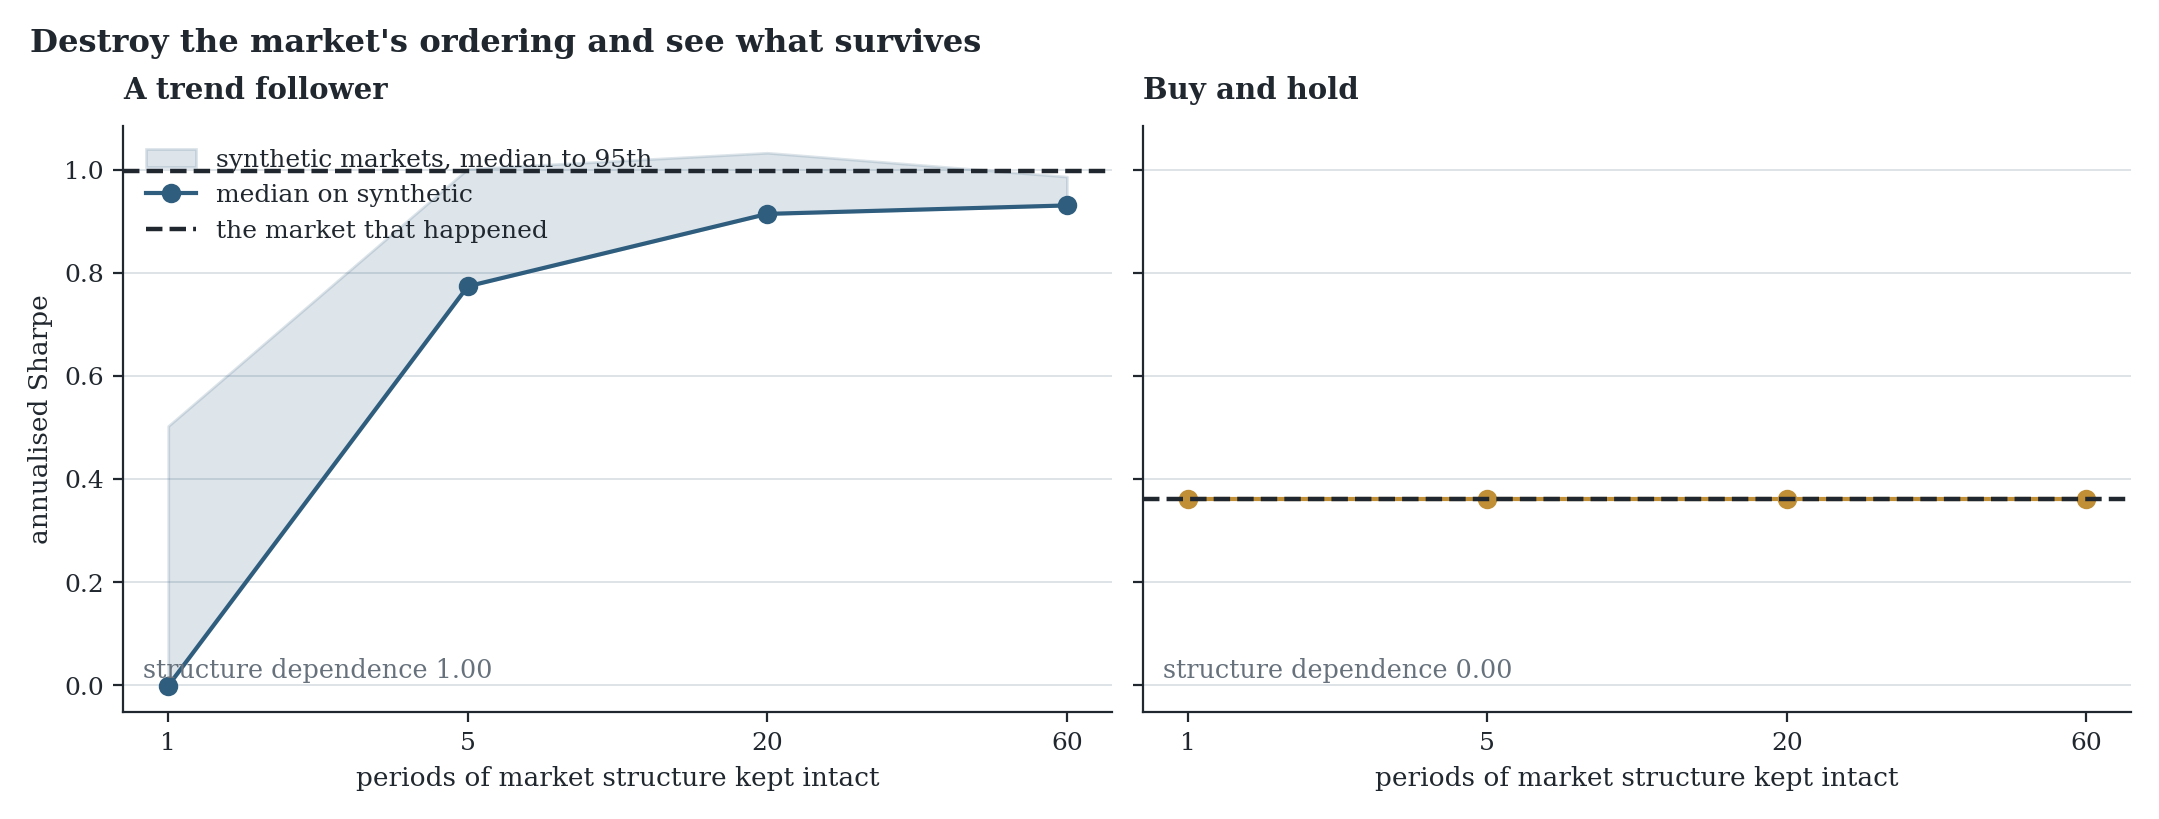
\includegraphics[width=\textwidth]{../docs/images/structure-sweep.png}
  \caption{\textbf{Two strategies on one market.} Both are rerun on 300 resampled histories at each block length. The trend follower needs the ordering and collapses without it. Buy and hold is unaffected at every block length, because reordering a series cannot change its mean or its standard deviation. Dashed lines mark the result on the market that actually happened.}
  \label{fig:sweep}
\end{figure}

\subsection{Relation to existing methods}

Resampling a series to break dependence and rerunning a procedure on the result goes back a long way. It is the surrogate-data method familiar from nonlinear time-series analysis, and it is closely related to permutation testing, to bootstrap inference for dependent data \citep{politis1994stationary,kunsch1989jackknife}, and to the data-snooping framework of \citet{white2000reality}, which resamples in order to build a null for the maximum over many models. What is offered here is narrower than a new method. It is the specific practice of sweeping $\ell$ rather than choosing one value, and reading the resulting curve as a statement about which kind of structure a result depends on. A single block length answers a single question. The gradient is what distinguishes the two cases below.

\section{What the curve separates}\label{sec:separates}

Figure~\ref{fig:sweep} runs the sweep on a simulated market with mild genuine momentum, $r_t = 0.06\,r_{t-1} + \varepsilon_t + \mu$, and two strategies.

The trend follower holds yesterday's direction. On the observed path it earns 1.00 annualised. At $\ell = 1$ the median across generated markets is 0.00 and the observed result exceeds every one of the 300 paths. As $\ell$ grows the synthetic markets regain the persistence the strategy trades, the median climbs to 0.77, 0.91 and 0.93, and the observed result stops being exceptional. Its structure dependence is $D = 1.00$.

This does not on its own establish a timing edge. A strategy whose exposure depends on recent realised variance, one with path-dependent position sizing, one with a lookback window that warms up differently on a reordered series, or one with an ordinary leakage bug will all collapse under shuffling in the same way. The sweep narrows the question from ``is this result real'' to ``this result requires the ordering, so what about the ordering is it using''. That is the claim the experiment supports, and it is smaller than it first looks.

Buy and hold earns 0.36 on the observed path and 0.36 at every block length, giving $D = 0.00$. The agreement is exact to within one floating point unit rather than approximate, because a permutation cannot change the multiset its result depends on. That is the correct answer rather than a failure of the method. Buy and hold earns from drift, drift is a property of the marginal distribution, and resampling preserves the marginal distribution exactly. A flat curve is informative. It says the result does not depend on when anything happened, which for a strategy that claims to time the market would be damning.

The recovery at large $\ell$ deserves emphasis, because it is easy to misread. A strategy scoring well on synthetic markets at $\ell = 60$ has not failed a test. Those markets contain the structure it exploits, by construction, so it should score well there. The evidence is the gradient, not any single level.

\section{Why the bootstrap is the wrong tool here}\label{sec:bootstrap}

The first version of this diagnostic used a stationary bootstrap, on the
reasoning that it is the standard resampling scheme for dependent data. That is
true, and it is still the wrong choice for this particular experiment.

A bootstrap draws with replacement. Some observations appear several times in a
generated path and others do not appear at all, so the path has a different
realised distribution from the source. Table~\ref{tab:bootstrap} measures the
size of that effect on 1500 draws from a Student $t$ with three degrees of
freedom, which is heavy tailed in roughly the way daily returns are.

\begin{table}[h]
  \centering
  \small
  \begin{tabular}{lr}
    \toprule
    Measured over 200 bootstrap paths & \\
    \midrule
    Distinct source values absent from a single path & 549 of 1500 \\
    Paths that lost the largest single loss entirely & 79 of 200 \\
    Skewness, source & $+0.298$ \\
    Skewness, one path & $+0.080$ \\
    Standard deviation of the path means & $3.97\times10^{-4}$ \\
    \bottomrule
  \end{tabular}
  \caption{How far a bootstrap path departs from the series it came from. The
  experiment is supposed to vary only the ordering, and these quantities do not
  depend on ordering at all.}
  \label{tab:bootstrap}
\end{table}

Every quantity in that table is order-invariant, so none of it should move in an
experiment about ordering. A strategy sensitive to tail behaviour could fail on
a bootstrap path because the tail it needed was not drawn, and the result would
be indistinguishable from a genuine dependence on sequence. That is the
confound, and it is silent.

The permutation removes the confound by construction rather than by argument, and
there is a sharp check available. Buy and hold depends only on the multiset of
returns, so its Sharpe ratio is a deterministic function of the data and cannot
move under any reordering. It is therefore a quantity whose correct behaviour is
known exactly in advance.

Over 4000 generated paths of a 2500 point series, the permutation returns the
source value every time, with a standard deviation of $1.6\times10^{-16}$. The
bootstrap returns a mean of $0.347$ against a source of $0.342$, which is $1.1$
standard errors and therefore consistent with no bias at all. The problem is not
the location. It is the spread. The bootstrap estimates scatter with a standard
deviation of $0.314$ on a quantity of $0.342$, so the noise it injects is the
same size as the thing being measured, into a statistic that cannot vary. Any
strategy tested this way inherits that noise, and a result can look dependent on
ordering when the ordering was never what moved it.

This is a trade and not a free improvement. The geometric block length in
\citet{politis1994stationary} exists to keep the resampled series stationary, and
permuting fixed blocks does not have that property. Permutation also joins blocks
that were never adjacent, which introduces discontinuities at the seams and
destroys dependence that spanned them. What is bought is an exactly fixed
marginal distribution. For a diagnostic whose entire question is whether
ordering matters, holding the distribution fixed is worth more than keeping the
path stationary. For interval estimation the ranking reverses, which is why the
package implements both.

The wider point is not about bootstraps. Any resampling scheme changes several
properties of a series at once unless it is chosen not to, and a diagnostic is
only as clean as the thing it holds fixed.

\section{On real markets}\label{sec:real}

Everything above runs on processes whose answer is fixed before the test starts, which is how one shows a measurement behaves as claimed and is not evidence about any market. This section is the run on real prices.

Five liquid exchange traded funds are used, SPY, QQQ, TLT, GLD and EEM, on daily adjusted closes from 2000 or from inception, between 5457 and 6683 observations each. Four strategies were fixed before the data was downloaded. Two of them, buy and hold and a one day reversal, have known behaviour, and disagreeing with them would have indicated a broken tool rather than a finding. The full table is distributed with the source.

Buy and hold returns $D = 0.00$ and $p = 1.000$ on all five series. This is the exactness argument of Section~\ref{sec:separates} holding on real returns with real fat tails rather than on a Gaussian simulation, and it is the check that exposed the tie handling defect described above. The one day reversal loses on every series and loses by more than nearly every arrangement of the same series, giving $D > 1$ throughout, which is what occurs when destroying the ordering improves a strategy. Short horizon reversal in daily equity returns is well documented and the sweep recovers it with the correct sign without being directed to look for it.

The two remaining strategies are the reason this section exists.

\begin{figure}[t]
  \centering
  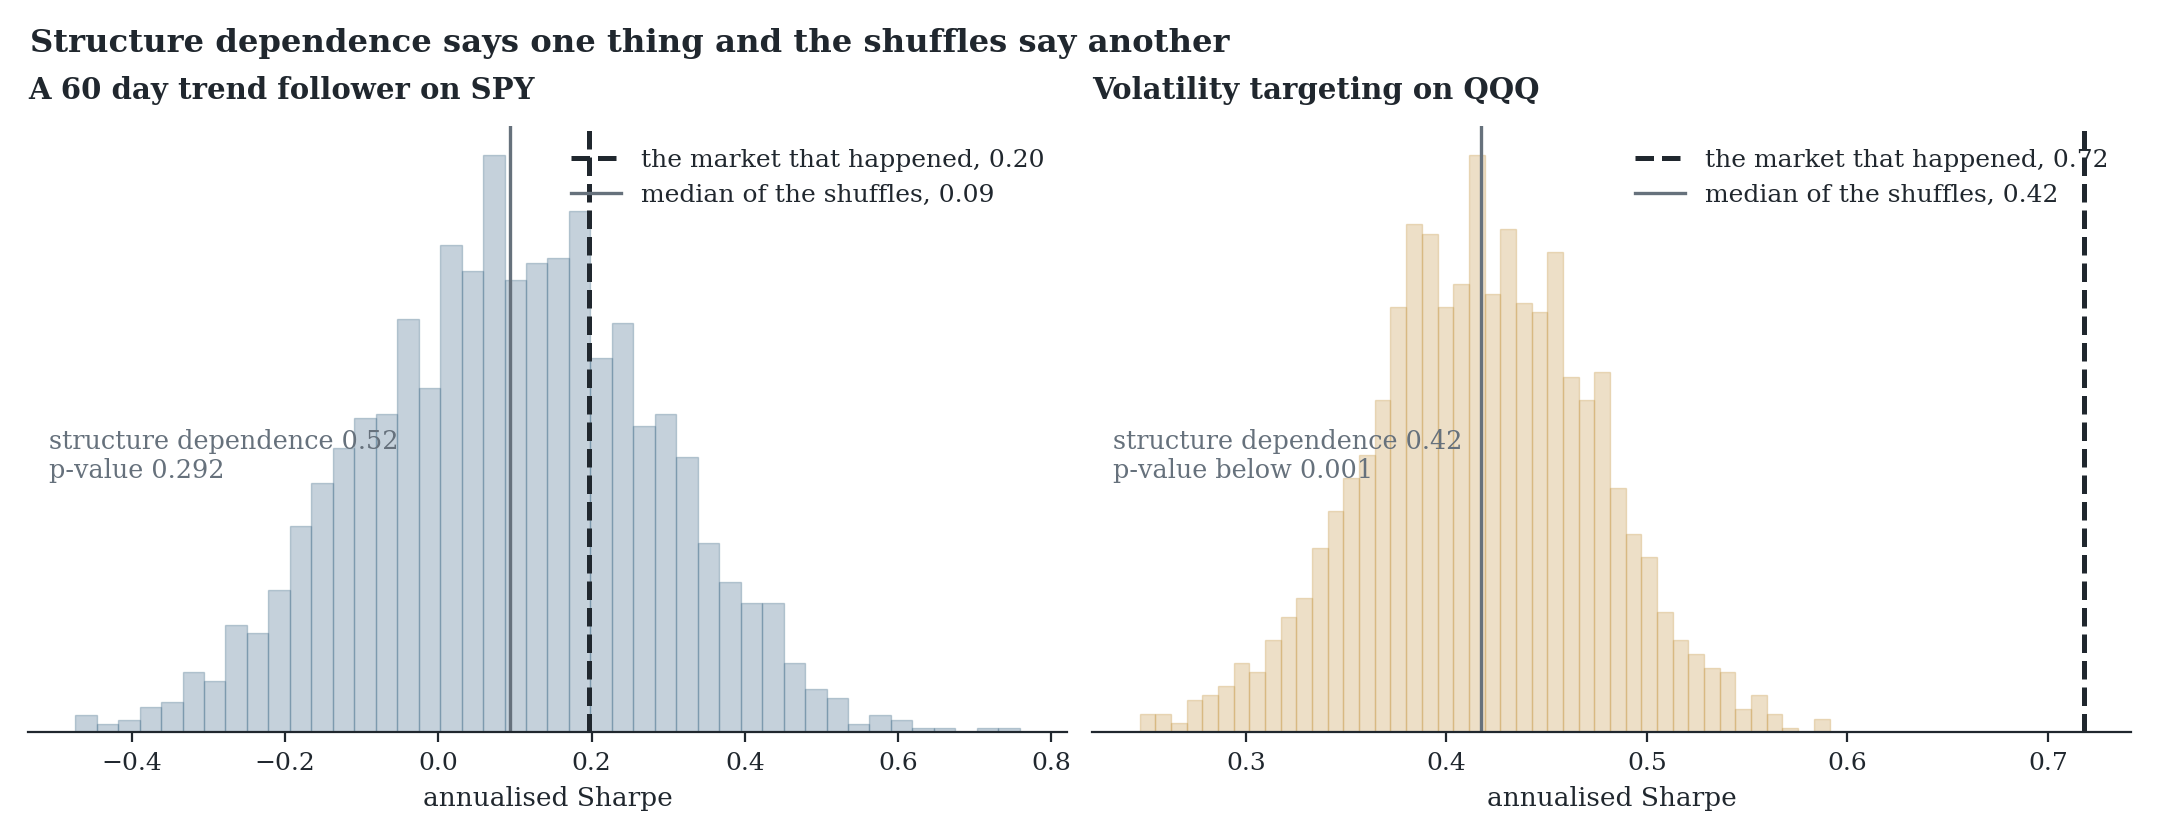
\includegraphics[width=\textwidth]{../docs/images/real-data.png}
  \caption{\textbf{The two summaries disagree, in both directions.} Each panel shows the Sharpe ratios of 2000 fully shuffled versions of the series, with the observed result dashed. Left, a 60 day trend follower on SPY, where the gap to the median is wide but the null is wider still. Right, volatility targeting on QQQ, where the gap is no larger and the null almost never reaches it.}
  \label{fig:real}
\end{figure}

A 60 day time series momentum rule returns $D$ between $0.52$ and $0.74$ across the five series, which read alone describes a strategy living entirely on the arrangement of history. Its p-value never falls below $0.18$. The shuffled markets reach its result between a fifth and two fifths of the time on every series tested. $D$ is large because the median shuffle earns very little, and $p$ is large because the shuffles are widely spread, and it is the spread that determines whether the gap carries information.

Volatility targeting produces the same disagreement in the opposite direction. It holds a long position at all times and varies only its size with trailing realised volatility, so it expresses no view on direction whatsoever. Its $D$ ranges from $0.07$ to $0.42$, uniformly small, because a position that stays long retains most of its Sharpe ratio when the returns are reordered. On QQQ not one of the generated markets reached its result, at either resolution run, giving $p = 0.002$ over 400 paths and $p = 0.0005$ over 2000. On SPY 11 of 400 reached it, giving $p = 0.030$. Volatility clusters, reducing exposure into that clustering is worth something measurable, and destroying the ordering removes it.

The two cases in Figure~\ref{fig:real} sit at $D = 0.52$ and $D = 0.42$, close enough to be treated as equivalent, with p-values of $0.29$ and $0.0005$. Neither is a timing edge. The trend follower does not clear chance on this data, and the volatility targeting clears it comfortably while having no directional view to be correct about. This is the claim of Section~\ref{sec:separates} arriving in a form that is harder to dismiss, because the strategy with the significant result is the one that most obviously is not forecasting anything.

\section{Implementation}\label{sec:implementation}

The library implements all three measurements in Python over NumPy and SciPy, and a subset in TypeScript for the browser interface. The two implementations of the expected-maximum-Sharpe expression and the inverse normal CDF agree to six decimal places on identical input, which is asserted in the test suite against reference values from SciPy rather than against each other.

Behaviour is tested rather than snapshotted. The suite asserts that independent resampling destroys autocorrelation while block resampling retains most of it, that a strategy with a genuine timing edge shows $D > 0.7$, and that a long-only strategy shows $D < 0.3$. Both implementations are required to place an order-invariant strategy at the exact centre of its null with $p = 1$, which is the assertion that would have caught the tie handling defect. Every generator is deterministic given a seed.

\section{Limitations}\label{sec:limitations}

\textbf{Exchangeable trials.} Both selection statistics assume the trials are roughly interchangeable draws. Searches that adapt, abandoning poor regions early, have an effective number of trials smaller than the number run, and both statistics will then be optimistic.

\textbf{The overfitting probability ignores time order.} It draws combinations of blocks without regard to which came first. A strategy that worked until a regime changed and then stopped is invisible to it. This is a property of the published method and it is the main reason it is not reported alone here.

\textbf{Volatility clustering survives only within blocks.} Real markets show persistence in volatility that outlives any practical block length, so the synthetic paths are calmer in the tails than the series they came from. A filtered resampling scheme that models conditional variance explicitly would improve this and is not implemented.

\textbf{No transaction costs.} A strategy trading at daily frequency can lose most of a 1.00 Sharpe ratio to spread and slippage. None of these measurements will register that, and a structure-dependence result says nothing about whether the edge survives execution.

\textbf{Five series is not a study.} Section~\ref{sec:real} uses real prices but tests four fixed strategies on five instruments in one asset class each. It is enough to demonstrate that the two summaries disagree in practice and to verify the exactness claim on real returns. It is not a survey of when they disagree, and no correction for testing four strategies on five series is applied to the p-values reported there.

\textbf{The null is arrangements, not markets.} Equation~\ref{eq:pvalue} asks how often a reordering of this history reaches the observed result. It does not ask how often a different history would, which is the question a practitioner usually wants and which no resampling of one path can answer.

\section{Conclusion}\label{sec:conclusion}

The number a backtest reports is real. What it measures is partly how hard you looked. The deflated Sharpe ratio and the probability of backtest overfitting both quantify that, and both are worth computing before anything else.

Neither tells you whether the market held anything to find. Destroying the ordering by degrees and rerunning the strategy does, and it separates two cases that a single Sharpe ratio cannot, a result that needs the arrangement of history and one that would have happened in any arrangement.

That separation needs two numbers rather than one. How much of the result the shuffling removes and how often the shuffling reaches it are different questions, and on real data they disagree in both directions. A strategy can lose most of its Sharpe ratio to shuffling and still be unremarkable against the shuffles, and one that loses little can be nearly unreachable. Neither pattern establishes a timing edge, and the second arose here from a rule with no directional view at all.

Passing all three is not evidence of an edge. It means selection alone does not explain the result, which is a much smaller claim, and the only one the arithmetic supports.

\bibliographystyle{plainnat}
\bibliography{references}

\end{document}
